\begin{surferPage}[Cubica de Cayley]{A C\'ubica de Cayley}
   Esta superf\'icie c\'ubica (superf\'icie de grau $3$) est\'a contida tamb\'em na galeria das superf\'icies simples. 
    Ao todo, ela tem quatro singularidades de cone duplo.
    Foi assim chamada em homenagem a Arthur Cayley que fez  investiga\c c\~ao  sobre c\'ubicas
    no s\'eculo XIX.
    
     No entanto, foi Ludwig Schl\"afli quem primeiro classificou estas superf\'icies em 1863 de forma sistem\'atica, no que diz respeito \`as suas poss\'iveis singularidades.
    Por exemplo, no  seu artigo pode ler-se porque raz\~ao n\~ao pode haver mais que $4$
    pontos singulares sobre uma superf\'icie c\'ubica. Este resultado permite concluir que  $\mu(3)=4$. 
    
    Por volta de 1900, Felix Klein estudou as formas poss\'iveis das superf\'icies c\'ubicas reais; a sua ideia era a de responder a essa  quest\~ao come\c cando pela C\'ubica de  Cayley e aplicando pequenas altera\c c\~oes:
    ao expandir as singularidades de cone duplo, desconectando ou fundindo partes,
Klein foi de facto capaz de encontrar todas as formas poss\'iveis.  Aqui est\~ao algumas delas:
    \vspace{0.3cm}
     \begin{center}
      \vspace{-0.2cm}
      \begin{tabular}{@{}c@{\ }c@{\ }c@{\ }c@{}}
        \begin{tabular}{@{}c@{}}
          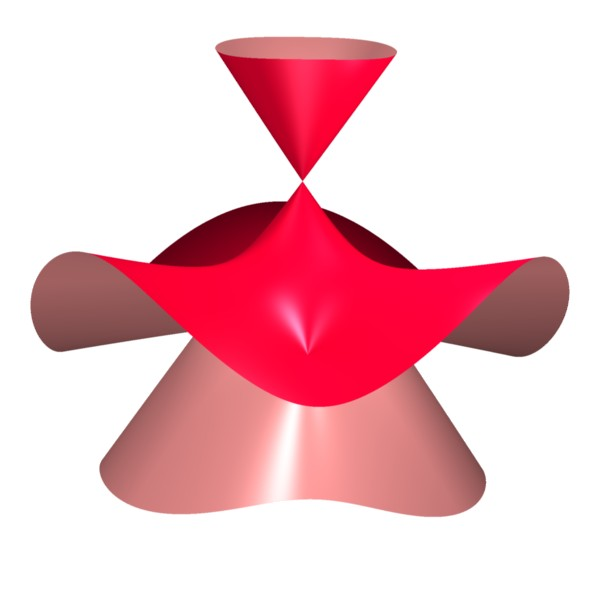
\includegraphics[width=1.35cm]{./../../common/images/cayley_cubic_0}
        \end{tabular}
        &
        \begin{tabular}{@{}c@{}}
          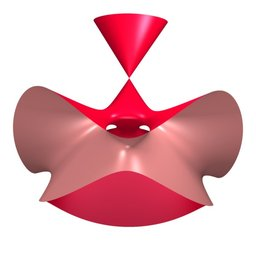
\includegraphics[width=1.35cm]{./../../common/images/cayley_cubic_1}
        \end{tabular}
        &
        \begin{tabular}{@{}c@{}}
          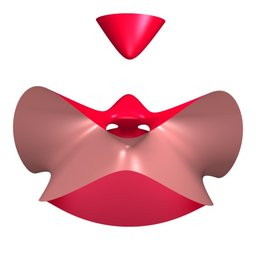
\includegraphics[width=1.35cm]{./../../common/images/cayley_cubic_2}
        \end{tabular}
        &
        \begin{tabular}{@{}c@{}}
          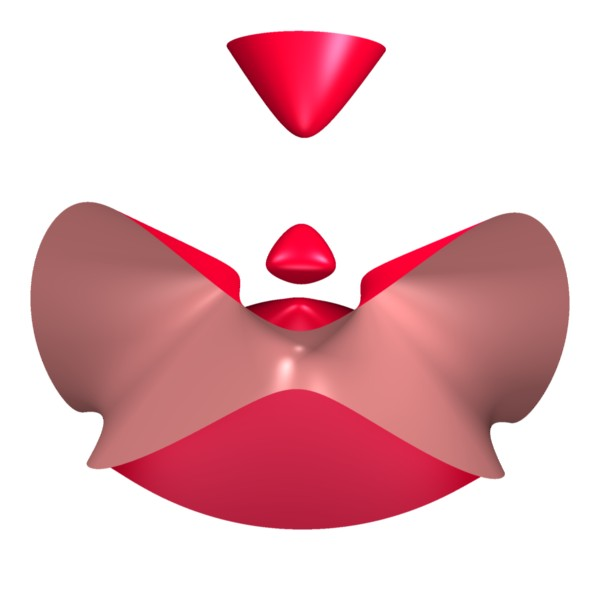
\includegraphics[width=1.35cm]{./../../common/images/cayley_cubic_3}
        \end{tabular}
      \end{tabular}
    \end{center}
\end{surferPage}
